\toclesssection{SCP 004 - The 12 Rusty Keys and the Door}
\addcontentsline{toc}{section}{SCP 004 - The 12 Rusty Keys and the Door}
\fakebold{Item \#:} SCP-004

\fakebold{Object Class:} Euclid

\begin{figure}[h]
\begin{center}
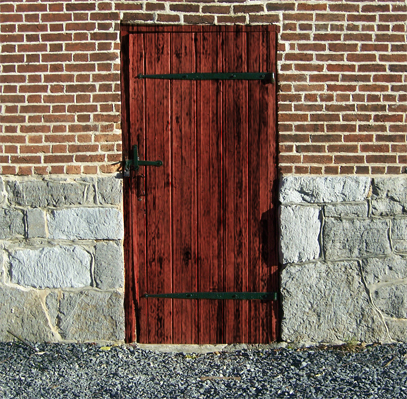
\includegraphics[scale=1.6]{scp/004.jpg}
\linebreak SCP-004-1
\end{center}
\end{figure}

\fakebold{Special Containment Procedures:} When handling items SCP-004-2 through SCP-004-13, proper procedure is vital. The items are not permitted off-site unless accompanied by two (2) Level 4 security personnel. Under no circumstances should any other component of SCP-004 be taken through SCP-004-1. The effects of doing so are as yet unknown, and the current cost of experimentation makes further research impractical. Should any of the objects contained within SCP-004-1 break containment, or the facility be breached, the keys must be brought inside and the door closed prior to activation of Site 62’s on-site warhead. Unauthorized removal of keys from the testing area is grounds for immediate termination.

Level 1 clearance is required for basic access to SCP-004-1; Level 4 clearance is required for use of SCP-004-2 to -13.

\fakebold{Description:} SCP-004 consists of an old wooden barn door (SCP-004-1) and a set of twelve (12) rusted steel keys (SCP-004-2 through SCP-004-13). The door itself is the entrance to an abandoned factory in \expunged.
\newpage

\begin{flushleft}
\fakebold{Chronological History}
\end{flushleft}
\fakebold{07/02/1949:} A group of three juveniles trespassing on federal property near \censor{XXXXXXXXXX} find the door. According to their testimony, they found a set of rusted keys in an iron lockbox and determined what door the keys unlock. The juveniles are taken into custody after they contact Sheriff \censor{XXXXXXXXXXXXXXXXX} when one of their friends (SCP-004-CAS01) goes missing.

\fakebold{07/03/1949:} Local authorities find the severed right hand of SCP-004-CAS01 eight kilometers from SCP-004-1. Other parts of SCP-004-CAS01's body are found scattered as far as 32 km from the factory. Under interrogation, the apprehended juveniles tell authorities that upon opening the door with one of the keys, SCP-004-CAS01 was torn into several pieces, each of which disappeared. At this point, the SCP Foundation takes over the investigation.

\fakebold{07/04/1949:} SCP Agent \censor{XXXXX} obtains the keys from the local authorities to begin testing. Tests show that SCP-004-2 through SCP-004-13 all fit into a single lock on the large barred door. 12 Class D personnel are assigned to test the effects of the door. Of the twelve (12) test subjects each trying a different key to enter the room, only two (2) survive. Opening the door with any key except SCP-004-7 or SCP-004-12 caused the test subjects to be torn apart in multiple directions; however, no dismembered parts were found until later. At the time of writing, only two (2) parts of each subject have been recovered (with the exception of the subject using SCP-004-\censor{X}, whose pieces were scattered in close proximity). The others have, for all intents and purposes, vanished from existence.

Of the two surviving subjects, only one (having used SCP-004-7) returned unharmed. The other came back in a near-catatonic state, able only to remove himself from the room and then collapse on the floor, and had to be restrained to prevent him from gouging out his eyes (see Appendix A: Mental Health Effects of SCP-004). The subject using SCP-004-7 said that he had entered a large room, impossibly big for the size of the attached building. After his exit, SCP-004-1 was propped open and an armed squad of Level 3 personnel entered. The size of the room is impossible to measure and the door frame and the individuals in the room are the only part of the room that can be felt or illuminated.

\fakebold{07/16/1949:} The juvenile suspects and Sheriff \censor{XXXXXXXXXXX} \censor{XXXXX} are terminated.

\fakebold{08/02/1949:} \censor{XXXXXXXXXXXXXXXXX} is declared a hazardous area "due to unexploded ordnance" and fences erected in order to prevent civilian ingress. Tests to determine safety of exposure to environment behind SCP-004-1 begin.

\fakebold{12/01/1950:} Space-time anomalies resulting from exposure to SCP-004 are confirmed. Testing is suspended until further notice.

\fakebold{07/03/19\censor{XX}:} The unaccounted-for remains of SCP-004-CAS01 appear unexpectedly outside SCP-004-1. Despite being killed decades before, the remains of SCP-004-CAS01 are not decomposed in any manner and are still warm to the touch. Blood remains uncoagulated. The remains are remanded for testing.

\fakebold{07/04/19\censor{XX}:} The unaccounted-for remains of one of the twelve (12) original test subjects appear in similar manner to those of SCP-004-CAS01. The remains have been designated SCP-004-CAS02. Records suggest that both SCP-004-CAS01 and CAS02 used SCP-004-\censor{XX}.

\fakebold{03/21/1999:} With the massive proliferation of nuclear weapons and World War III only \censor{XX} years away, construction has begun on a site inside SCP-004-1. The site is to stock supplies for \censor{XXXXXXX} person-days.

\fakebold{04/21/1999:} \censor{XXXXXXXXXXXXXXXXX} has ordered the site inside SCP-004-1 to be expanded to include emergency storage for all mobile SCP-\censor{XXX} specimens and a \censor{XX}-petabyte database for the storage of all SCP data. The facility is now referred to as Site-62.

\fakebold{09/25/2000:} Site-62 is operational. Labs and containment units are complete and can contain the most dangerous specimens. Backup of the SCP database has begun.

\fakebold{01/25/2001:} Due to time anomalies (see “Space-Time Anomalies” below), all personnel working at Site-62 are now required to reside on-site permanently. Families of personnel are to be informed that loved ones perished in an industrial accident. Cloned bodies have been prepared for funeral.

\fakebold{07/14/2003:} Massive power outage across Northeast United States and through Canada. Due to the initial failure of multiple SCP generators, Site-62 was without power for fifty-three (53) minutes. During those fifty-three (53) minutes, those on site were completely without any source of light. They reported "sensing" creatures and people, although no abnormal entities could be seen or felt. Selected facility personnel were allowed to read \censor{XXXXXXXXXXXX} (Appendix A) and said the creatures "sensed" were of humanoid size but otherwise similar to the massive green creature described.

\begin{flushleft}
\fakebold{Space-Time Anomalies}
\end{flushleft}

SCP-004 seems to propagate spatiotemporal anomalies. Personnel leaving the facility report losing time. Those who have been in the site for weeks insist that they had only been in the facility for several days, and records of work completed and supplies consumed support their claims. Other temporal anomalies involve SCP-004-2 through -13, especially the reappearance of SCP-004-CAS01 and SCP-004-CAS02 exactly \censor{XX} years after using SCP-004-\censor{XX}. \censor{XXXXXXXXXXXXXXXXXXXX} has been assigned to investigate all aspects of these time anomalies. Spatial anomalies include the impossibly large dimensions of the area opened by SCP-004-7. Similarly, the 2003 blackout incident suggests that there exists an alternate plane of existence within the same space that Site-62 occupies.

\begin{flushleft}
\fakebold{Further Notes}
\end{flushleft}

Testing on SCP-004 reveals that ten (10) of the keys open SCP-004-1 on a dimension where the laws of physics and topology are significantly different than those of our home dimension. Test subjects meeting these hostile conditions are torn apart, their body parts deposited in various locations, only three of which have been verified to be on Earth. Material deposited at two of these points appears immediately; material deposited at the third appears exactly \censor{XX} years into the future. The other seven locations are currently unknown.
\newpage
Current testing focuses on two avenues of research. The first is finding ways to survive SCP-004’s hostile topologies. The second \expunged \ suggest that SCP-004-2 through -13 may open doors other than SCP-004-1.

\begin{flushleft}
\fakebold{Appendix A: Mental Health Effects of SCP-004-12}
\end{flushleft}

All Class D personnel using SCP-004-12 return in a catatonic state, unable to speak. Some may have enough energy left to try to claw out their eyes. Of the 16 subjects, only 4 have survived. Only one has regained speech, following long-term psychotherapy. He was able to tell the psychiatrist that he saw a massive green creature, so large that much of its body extended beyond his field of view. He reported innate fear and sudden recognition, “as if it were something buried deep in \lb his\rb \ primal fears,” and forced implantation of “incomprehensible” memories. Subject displays acute anterograde and retrograde amnesia.

\begin{flushleft}
\fakebold{Appendix B}
\end{flushleft}

\fakebold{Item \#:} SCP-004-14

\fakebold{Date of Discovery:} 09/02/1950

\fakebold{Origin of Object:} Object was discovered elsewhere in factory area, in the previously undiscovered manager's office.

\fakebold{Description:} Object appears as a large (182 cm X 129 cm), unvarnished wooden box. The box may be unlocked by the "safe" key, SCP-004-7, as well as five of the "unsafe" keys (see Document SCP-004-1).

Upon unlocking SCP-004-14 with SCP-004-7, the box opens automatically on hinges. The volume of the space inside is precisely five times greater than the outer dimensions imply. Items placed within while the lid remains open do not affect the weight or any other properties of the box. When the lid is closed and locked, however, all items inside vanish irretrievably. Personnel locked inside the box are also irretrievable, although losing personnel in this fashion appears to affect significantly the dreams experienced by \expunged.